\documentclass{ximera}

\graphicspath{{./}{thePythagoreanTheorem/}{deMoivreSavesTheDay/}{complexNumbersFromDifferentAngles/}}

\usepackage{tikz}
\usepackage{tkz-euclide}
\usetkzobj{all}
\tikzstyle geometryDiagrams=[ultra thick,color=blue!50!black]
\newcommand{\tri}{\triangle}
\renewcommand{\l}{\ell}
\renewcommand{\P}{\mathcal{P}}
\newcommand{\R}{\mathbb{R}}
\newcommand{\Q}{\mathbb{Q}}

\newcommand{\Z}{\mathbb Z}

\renewcommand{\vec}{\mathbf}
\renewcommand{\d}{\,d}



%% Egyptian symbols

\usepackage{multido}
\newcommand{\egmil}[1]{\multido{\i=1+1}{#1}{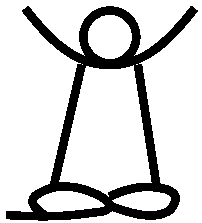
\includegraphics[scale=.1]{egyptian/egypt_person.pdf}\hspace{0.5mm}}}
\newcommand{\eghuntho}[1]{\multido{\i=1+1}{#1}{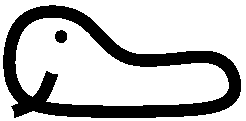
\includegraphics[scale=.1]{egyptian/egypt_fish.pdf}\hspace{0.5mm}}}
\newcommand{\egtentho}[1]{\multido{\i=1+1}{#1}{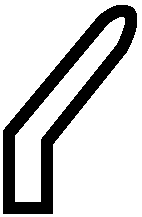
\includegraphics[scale=.1]{egyptian/egypt_finger.pdf}\hspace{0.5mm}}}
\newcommand{\egtho}[1]{\multido{\i=1+1}{#1}{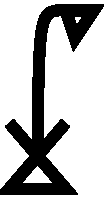
\includegraphics[scale=.1]{egyptian/egypt_lotus.pdf}\hspace{0.5mm}}}
\newcommand{\eghun}[1]{\multido{\i=1+1}{#1}{
\includegraphics[scale=.1]{egyptian/egypt_scroll.pdf}\hspace{0.5mm}}}
\newcommand{\egten}[1]{\multido{\i=1+1}{#1}{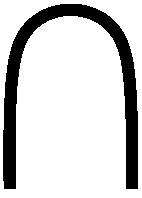
\includegraphics[scale=.1]{egyptian/egypt_heel.pdf}\hspace{0.5mm}}}
\newcommand{\egone}[1]{\multido{\i=1+1}{#1}{
\includegraphics[scale=.1]{egyptian/egypt_stroke.pdf}\hspace{0.5mm}}}
\newcommand{\egyptify}[7]{
 \multido{\i=1+1}{#1}{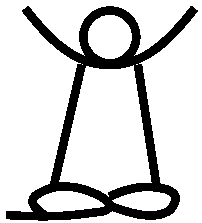
\includegraphics[scale=.1]{egyptian/egypt_person.pdf}\hspace{0.5mm}}
 \multido{\i=1+1}{#2}{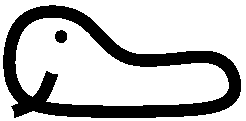
\includegraphics[scale=.1]{egyptian/egypt_fish.pdf}\hspace{0.5mm}}
 \multido{\i=1+1}{#3}{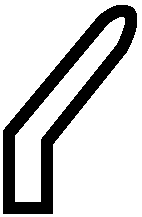
\includegraphics[scale=.1]{egyptian/egypt_finger.pdf}\hspace{0.5mm}}
 \multido{\i=1+1}{#4}{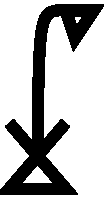
\includegraphics[scale=.1]{egyptian/egypt_lotus.pdf}\hspace{0.5mm}}
 \multido{\i=1+1}{#5}{
\includegraphics[scale=.1]{egyptian/egypt_scroll.pdf}\hspace{0.5mm}}
 \multido{\i=1+1}{#6}{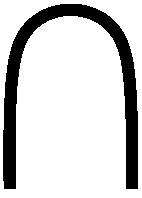
\includegraphics[scale=.1]{egyptian/egypt_heel.pdf}\hspace{0.5mm}}
 \multido{\i=1+1}{#7}{
\includegraphics[scale=.1]{egyptian/egypt_stroke.pdf}\hspace{0.5mm}}
 \hspace{.5mm}
}




\title{Newton and Kepler}

\begin{document}
\begin{abstract}
In this activity we deduce Kepler's second law of planetary motion
from Newton's theory of gravitation.
\end{abstract}
\maketitle

In 1686, Isaac Newton published his book \textit{Philosophi\ae\
Naturalis Principia Mathematica}. This book contained Newton's theory
of gravitation:
\[
F = \frac{GMm}{R^2}
\] 
where $F$ is the magnitude of the force exerted between the masses, $M$ is the first (larger) mass, $m$ is the second (smaller) mass, $G$ is the gravitational constant, and $R$ is the distance between the centers of the masses. 

On the other hand in 1609, Kepler published his \textit{Second Law of
Planetary Motion}. This law states:
\begin{quote}
A line joining a planet and the Sun sweeps out equal areas during
equal intervals of time.
\end{quote}

One of the triumphs of Newton's theory of gravitation is that one can
actually deduce Kepler's laws (including the Second Law) from this
theory, Newton's \textit{Second Law of Motion}, and a bit of vector
calculus. Let's see how it's done. Note, we are giving a modern proof,
not the one Newton gave himself.

\begin{question}
Start with Newton's second law of motion, and explain the equation below:
\[
\vec{F} = m \vec{a} = m \frac{d^2\vec{R}}{dt^2} = \frac{-GMm}{|\vec{R}|^2}\cdot \frac{\vec{R}}{|\vec{R}|}
\]
\end{question}

\begin{question}
Explain why $\frac{d^2\vec{R}}{dt^2}$ is proportional to $\vec{R}$.
\end{question}

\begin{question}
Explain why 
\[
\vec{R} \times \frac{d^2\vec{R}}{dt^2} = \vec{0}.
\]
\end{question}

\begin{question}\label{Q:removeNaught}
Compute:
\[
\frac{d}{dt}\left(\vec{R}\times \frac{d\vec{R}}{dt}\right)
\]
and let:
\[
\vec{R}\times \frac{d\vec{R}}{dt}=\vec{C}
\]
What can you conclude about $\vec{C}$?
\end{question}


\begin{question}
Explain why $\vec{v}=\frac{d\vec{R}}{dt}$ and $\vec{R}$ lie in a plane
orthogonal to vector $\vec{C}$.
\end{question}

Let the plane containing $\vec{v}$ and $\vec{R}$ be the
$(x,y)$-plane. Let $\vec{k}$ be a unit vector in the direction of
$\vec{C}$. We will now switch to polar coordinates, where $t=0$ and
$\theta=0$ give direction of $\vec{R}$ when $|\vec{R}|$ is at a
minimum. Let $\vec{R}_0$ and $\vec{v}_0$ be the vector and velocity
corresponding to this minimum distance.

\begin{question}
Explain why 
\[
\vec{C} = \vec{R}_0\times \vec{v}_0.
\]
\end{question}


\begin{question}
Recalling that in polar coordinates
\begin{enumerate}
\item $\vec{R} = r\vec{u}_r$
\item $\vec{v} = \vec{u}_r \frac{dr}{dt} + \vec{u}_\theta \cdot r \frac{d\theta}{dt}$
\end{enumerate}
where (as usual for polar coordinates) $\vec{u}_r$ is a unit vector
pointing in the direction of the radius and $\vec{u}_\theta$ is a unit
vector perpendicular to the radius. Explain why
\[
\vec{C}=\vec{R}_0\times \vec{v}_0 = \vec{k} \left[r^2 \frac{d\theta}{dt}\right]_{t=0}= \vec{k} \cdot r_0v_0.
\]
\end{question}

\begin{question}
Now use Question~\ref{Q:removeNaught} to conclude
\[
\vec{k} \cdot r^2 \frac{d\theta}{dt}= \vec{k} \cdot r_0v_0
\]
\end{question}



\begin{question}
Recall in polar coordinates that area, $A$, is given by
\[
A = \frac{1}{2}\int_{\theta_0}^{\theta_1} r^2\d\theta. 
\]
Explain why if $\theta$ and $r$ are both functions of $t$, with
$\theta_0 = \theta(t_0)$ and $\theta_1 = \theta(t_1)$,
\[
A =  \frac{1}{2}\int_{\theta_0}^{\theta_1} r^2\d\theta = \frac{1}{2}\int_{t_0}^{t_1} r^2 \frac{d\theta}{dt} \d t 
\]
\end{question}


\begin{question}
Explain how this proves Kepler's Second Law:
\begin{quote}
A line joining a planet and the Sun sweeps out equal areas during equal intervals of time.
\end{quote}
Exactly which facts about the gravitational force did we use?
\end{question}
\end{document}
